\documentclass[conference]{IEEEtran}
\IEEEoverridecommandlockouts
\usepackage{cite}
\usepackage{amsmath,amssymb,amsfonts,amsthm}
\usepackage{algorithmic}
\usepackage{algorithm}
\usepackage{graphicx}
\usepackage{textcomp}
\usepackage{xcolor}
\usepackage{booktabs}
\usepackage{multirow}
\usepackage{tikz}
\usepackage{subcaption}
\usetikzlibrary{patterns,arrows.meta,positioning,calc}

\newtheorem{theorem}{Theorem}
\newtheorem{lemma}[theorem]{Lemma}
\newtheorem{definition}{Definition}

\def\BibTeX{{\rm B\kern-.05em{\sc i\kern-.025em b}\kern-.08em
    T\kern-.1667em\lower.7ex\hbox{E}\kern-.125emX}}

\begin{document}

\title{Dynamic Platoon Formation of Multi-Type Autonomous Vehicles for Sustainable Urban Mobility}

\author{
\IEEEauthorblockN{Jaeyun Ree}
\IEEEauthorblockA{
\textit{Faculty of Information Technology} \\
\textit{Monash University} \\
Melbourne, VIC, Australia \\
jree0010@student.monash.edu
}
\and
\IEEEauthorblockN{Mohammed Eunus Ali}
\IEEEauthorblockA{
\textit{Faculty of Information Technology} \\
\textit{Monash University} \\
Melbourne, VIC, Australia \\
eunus.ali@monash.edu
}
}

\maketitle

\begin{abstract}
This paper addresses the energy inefficiency of single-occupancy vehicles by introducing a novel cooperative autonomous vehicle system where smaller Passive Vehicles (PVs) can be physically towed by larger Active Vehicles (AVs) during shared highway segments. Unlike traditional platooning that relies solely on aerodynamic drafting, our approach enables propulsion energy elimination for towed vehicles during attached segments. We formulate the platoon formation problem as a constrained optimization problem on a one-dimensional highway model and propose two algorithms: a Greedy Maximum-Weight Matching algorithm and an Iterative Linear Assignment (ILA) algorithm using the Jonker--Volgenant method. A key innovation is the multi-segment matching capability, allowing a single PV to be towed by multiple AVs across different route segments. Experimental evaluation on synthetic scenarios with up to 400 PVs and 80 AVs demonstrates that both algorithms achieve 25--52\% distance coverage (proportional to energy savings under constant per-distance propulsion) depending on capacity, with ILA providing per-iteration optimality (optimal solutions to each bipartite subproblem) and superior runtime performance (5--15$\times$ faster) due to highly optimized compiled implementations.
\end{abstract}

\begin{IEEEkeywords}
autonomous vehicles, vehicle platooning, energy efficiency, Hungarian algorithm, combinatorial optimization, intelligent transportation systems
\end{IEEEkeywords}

%==============================================================================
% SECTION 1: INTRODUCTION
%==============================================================================
\section{Introduction}

% Paragraph 1: High-level motivation (world problem + statistics)
The persistent over-reliance on single-occupancy vehicles poses significant challenges to urban transportation sustainability. According to the U.S. Department of Transportation's National Household Travel Survey, drive-alone trips account for the vast majority of commute travel, contributing substantially to traffic congestion, energy consumption, and carbon emissions~\cite{usdot2022}. The transportation sector alone is responsible for nearly 29\% of total greenhouse gas emissions in the United States, with light-duty vehicles contributing the largest share~\cite{epa2023}. This inefficiency is particularly pronounced along shared routes where multiple individuals travel similar paths yet operate their vehicles independently.

% Paragraph 2: Problem and idea (platooning/cooperation concept)
Autonomous vehicle (AV) technology presents a transformative opportunity to address these challenges through coordinated vehicle operation. This paper introduces a novel concept of \textit{active} and \textit{passive} autonomous vehicles, where smaller Passive Vehicles (PVs) can temporarily attach to larger Active Vehicles (AVs) during shared highway segments. Unlike traditional vehicle platooning that maintains physical separation between vehicles, our approach enables physical coupling where a PV's propulsion system is deactivated while being towed, eliminating propulsion energy consumption for the towed vehicle during attached segments. In our model, we abstract energy savings as proportional to distance covered while towed; extending to physics-based energy models incorporating rolling resistance and aerodynamic drag is left for future work. This paradigm shifts transportation from isolated driving to an on-demand, energy-transfer-based mobility service.

% Paragraph 3: Related work sketch and differentiation
Existing research on cooperative vehicle systems spans several related but distinct areas. Traditional platooning systems~\cite{tsugawa2016review,bergenhem2012overview} focus on coordinated driving with aerodynamic benefits, typically achieving 10--20\% fuel savings through drafting. Ridesharing and carpooling optimization~\cite{furuhata2013ridesharing,agatz2012optimization} address passenger matching but not vehicle coupling. Eco-driving strategies~\cite{sciarretta2020energy,hellstrom2009look} optimize individual vehicle behavior without inter-vehicle coordination. The assignment problem we address relates to the classic bipartite matching literature~\cite{kuhn1955hungarian,munkres1957algorithms}, though our multi-segment matching with capacity constraints introduces novel complexity. While these approaches offer incremental improvements, they do not address the fundamental inefficiency of independent propulsion for vehicles with overlapping routes.

% Paragraph 4: Our solution summary (big picture)
We formulate the platoon formation problem on a one-dimensional highway model where the objective is to maximize total distance coverage (as a proxy for energy savings) through strategic PV-to-AV assignments. To solve this problem, we propose two complementary algorithms. The \textit{Greedy Maximum-Weight Matching} algorithm provides an intuitive baseline through iterative selection, while the \textit{Iterative Linear Assignment (ILA)} algorithm using SciPy's \texttt{linear\_sum\_assignment} (Jonker--Volgenant algorithm~\cite{scipy2020}) guarantees optimal solutions per iteration. Surprisingly, our experiments reveal that ILA is not only optimal but also faster (5--15$\times$) due to highly optimized compiled C implementations that avoid the repeated sorting overhead inherent in greedy approaches. A key innovation is our multi-segment matching capability: rather than restricting each PV to a single AV, our algorithms allow a PV to be towed by different AVs across different segments of its route.

% Paragraph 5: Contributions (what we show in results)
The main contributions of this paper are:
\begin{itemize}
    \item A formal one-dimensional problem formulation that captures the essential trade-offs in cooperative vehicle platooning, including multi-segment matching and point-wise capacity constraints.
    \item A Greedy algorithm that serves as an intuitive baseline with empirically competitive performance.
    \item An Iterative Linear Assignment (ILA) algorithm using the Jonker--Volgenant method~\cite{scipy2020} that achieves per-iteration optimality with capacity constraints via virtual slot expansion.
    \item Multi-segment matching capability allowing PVs to be towed by multiple AVs across their routes, with point-wise capacity tracking at each highway position.
    \item Comprehensive experimental evaluation on scenarios with 50--80 AVs, 200--400 PVs, demonstrating 25--52\% distance coverage savings.
\end{itemize}

%==============================================================================
% SECTION 2: RELATED WORK
%==============================================================================
\section{Related Work}

\subsection{Vehicle Platooning}

Vehicle platooning has received significant attention in both academia and industry. Tsugawa et al.~\cite{tsugawa2016review} provide a comprehensive review of truck platooning projects, reporting fuel savings of 10--20\% through aerodynamic drafting. The PATH project~\cite{shladover2009cooperative} demonstrated automated highway systems with close-following platoons. The European project SARTRE~\cite{bergenhem2012overview} explored multi-brand platooning for commercial vehicles with heterogeneous manufacturers.

However, all existing platooning approaches maintain physical separation between vehicles---the ``platoon'' is virtual, maintained through V2V communication and coordinated control. Our approach fundamentally differs by enabling \textit{physical coupling}, where smaller vehicles are towed by larger ones. In our simplified model, this eliminates PV propulsion energy during towing segments; system-level energy analysis incorporating AV towing load is deferred to future work.

\subsection{Ridesharing and Vehicle Routing}

The ridesharing literature addresses matching passengers to vehicles~\cite{furuhata2013ridesharing,agatz2012optimization}. Dynamic ride-sharing systems~\cite{alonso2017demand} optimize real-time matching with capacity constraints. The dial-a-ride problem~\cite{cordeau2007dial} considers pickup and delivery with time windows. While these problems share structural similarities (matching with constraints), they focus on passenger-to-vehicle assignment rather than vehicle-to-vehicle coupling.

\subsection{Assignment and Matching Problems}

Our problem relates to classic assignment problems. The Hungarian algorithm~\cite{kuhn1955hungarian,munkres1957algorithms} solves bipartite matching optimally in $O(n^3)$ time. Extensions to capacitated assignment~\cite{burkard2012assignment} handle agents with multiple slots. The generalized assignment problem~\cite{cattrysse1992survey} addresses heterogeneous costs and capacities.

Our contribution extends this literature by introducing: (1) multi-segment matching where one agent (PV) can be served by multiple providers (AVs) across different segments, and (2) point-wise capacity constraints where an AV's available capacity varies along its route as PVs attach and detach.

\subsection{Cooperative Autonomous Vehicles}

Recent work on cooperative autonomous vehicles explores coordination mechanisms beyond platooning. Cooperative adaptive cruise control (CACC)~\cite{ploeg2011design} enables string-stable following. Intersection management~\cite{dresner2008multiagent} coordinates crossing without traffic signals. These coordination mechanisms focus on maintaining separation while our work addresses physical coupling.

Our work introduces a new cooperation paradigm: physical towing between heterogeneous vehicle types. This requires solving a novel matching problem with spatial and temporal constraints not present in existing cooperative driving literature.

%==============================================================================
% SECTION 3: PROBLEM DEFINITION
%==============================================================================
\section{Problem Formulation}

We formalize the platoon formation problem on a simplified one-dimensional highway model. This abstraction captures the essential optimization trade-offs while enabling tractable analysis. Extension to general road networks is discussed in Section~\ref{sec:future}.

\subsection{Notation Summary}

Table~\ref{tab:notation} summarizes the key notation used throughout this paper.

\begin{table}[htbp]
\caption{Summary of Notation}
\label{tab:notation}
\centering
\begin{tabular}{cl}
\toprule
\textbf{Symbol} & \textbf{Description} \\
\midrule
$L$ & Highway length \\
$\mathcal{A}$ & Set of Active Vehicles (AVs), $|\mathcal{A}| = N$ \\
$\mathcal{P}$ & Set of Passive Vehicles (PVs), $|\mathcal{P}| = M$ \\
$e_i^a, x_i^a$ & Entry and exit points of AV $a_i$ \\
$e_j^p, x_j^p$ & Entry and exit points of PV $p_j$ \\
$C_i$ & Towing capacity of AV $a_i$ \\
$t_i^a, v_i^a$ & Entry time and speed of AV $a_i$ \\
$d_{ij}$ & Shared travel distance between $a_i$ and $p_j$ \\
$S_{ij}$ & Energy saving when $p_j$ is towed by $a_i$ \\
$cp_{ij}, dp_{ij}$ & Coupling and decoupling points \\
$L_{min}$ & Minimum shared distance for platooning \\
$\tau$ & Time tolerance for coupling synchronization \\
\bottomrule
\end{tabular}
\end{table}

\subsection{System Model}

We consider a coordinated platoon formation system operating on a unidirectional highway segment of length $L$. The system comprises two distinct vehicle classes.

\begin{definition}[Active Vehicle]
An Active Vehicle (AV) $a_i \in \mathcal{A}$ is a larger autonomous vehicle capable of towing multiple smaller vehicles. Each AV is characterized by the tuple $(e_i^a, x_i^a, C_i, t_i^a, v_i^a)$ where $e_i^a, x_i^a \in [0, L]$ are entry and exit points, $C_i \in \mathbb{Z}^+$ is the towing capacity, and $t_i^a, v_i^a$ are the entry time and constant speed.
\end{definition}

\begin{definition}[Passive Vehicle]
A Passive Vehicle (PV) $p_j \in \mathcal{P}$ is a smaller autonomous vehicle that can be towed by AVs. Each PV is characterized by the tuple $(e_j^p, x_j^p, t_j^p, v_j^p)$ where $e_j^p, x_j^p \in [0, L]$ are entry and exit points, and $t_j^p, v_j^p$ are entry time and self-driving speed.
\end{definition}

\subsection{Shared Path and Energy Model}

For an AV $a_i$ and PV $p_j$, the \textit{shared path} is the overlap of their routes:
\begin{equation}
    d_{ij} = \max(0, \min(x_i^a, x_j^p) - \max(e_i^a, e_j^p))
    \label{eq:shared}
\end{equation}

The coupling point $cp_{ij}$ (where PV attaches) and decoupling point $dp_{ij}$ (where PV detaches) are:
\begin{align}
    cp_{ij} &= \max(e_i^a, e_j^p) \label{eq:cp}\\
    dp_{ij} &= \min(x_i^a, x_j^p) \label{eq:dp}
\end{align}

The energy saving $S_{ij}$ when PV $p_j$ is towed by AV $a_i$ is proportional to the shared distance:
\begin{equation}
    S_{ij} = \alpha \cdot d_{ij}
    \label{eq:saving}
\end{equation}
where $\alpha$ is an energy coefficient. For simplicity, we set $\alpha = 1$, making energy saving equivalent to distance saved.

\subsection{Multi-Segment Matching}

A key innovation of our formulation is \textit{multi-segment matching}: a single PV can be matched to multiple AVs across different segments of its route.

\begin{definition}[Segment Assignment]
A segment assignment for PV $p_j$ to AV $a_i$ is a tuple $(p_j, a_i, s, e)$ where $[s, e] \subseteq [e_j^p, x_j^p]$ is the segment during which $p_j$ is towed by $a_i$.
\end{definition}

For PV $p_j$, its route from $e_j^p$ to $x_j^p$ can be partitioned into segments:
\begin{itemize}
    \item \textit{Covered}: PV is towed by an AV (energy saved)
    \item \textit{Uncovered}: PV drives independently (no energy saved)
\end{itemize}

\textbf{Progressive Coverage Assumption:} Our algorithms process towing segments in spatial order along the highway. Each PV maintains a \textit{current left boundary} $\ell_j$ (initially $e_j^p$) representing the leftmost uncovered position. When PV $p_j$ is assigned to AV $a_i$, the towing segment starts at $\max(e_i^a, \ell_j)$ and $\ell_j$ advances to the decoupling point. This ensures uncovered regions are always contiguous suffix intervals $[\ell_j, x_j^p]$, simplifying state management while capturing the natural left-to-right progression of vehicles along the highway.

\subsection{Optimization Problem}

Let $\mathcal{X}$ denote the set of all segment assignments $(p_j, a_i, s, e)$ where PV $p_j$ is towed by AV $a_i$ over segment $[s, e]$. The optimization problem is:

\begin{align}
    \max \quad & \sum_{(p_j, a_i, s, e) \in \mathcal{X}} (e - s) \label{eq:obj}\\
    \text{s.t.} \quad & \left|\{(p_j, a_i, s, e) \in \mathcal{X} : x \in [s, e]\}\right| \leq C_i \notag\\
    & \qquad \forall i \in [N], \forall x \in [e_i^a, x_i^a] \label{eq:capacity}\\
    & \text{Segments for each } p_j \text{ are pairwise disjoint} \label{eq:nonoverlap}\\
    & (e - s) \geq L_{min} \quad \forall (p_j, a_i, s, e) \in \mathcal{X} \label{eq:minlen}
\end{align}

\textbf{Constraint Interpretation:}
\begin{itemize}
    \item \textbf{Point-wise Capacity} \eqref{eq:capacity}: At any position $x$ along AV $a_i$'s route, the number of simultaneously towed PVs cannot exceed $C_i$. This is the key constraint that distinguishes our problem from standard bipartite matching---an AV's effective capacity varies along its route as PVs attach and detach.
    \item \textbf{Non-overlap} \eqref{eq:nonoverlap}: A PV cannot be towed by two AVs simultaneously at any position.
    \item \textbf{Minimum length} \eqref{eq:minlen}: Each towing segment must exceed $L_{min}$ to justify coupling overhead.
\end{itemize}

\begin{lemma}[Critical Points Sufficiency]
\label{lem:critical}
Fix an AV $a_i$ and let $\mathcal{X}_i = \{(p_j, a_i, s, e) \in \mathcal{X}\}$ be the assignments to $a_i$. Define the critical set $\mathcal{C}_i = \{e_i^a, x_i^a\} \cup \{s, e : (p_j, a_i, s, e) \in \mathcal{X}_i\}$. Then the point-wise capacity constraint \eqref{eq:capacity} holds for all $x \in [e_i^a, x_i^a]$ if and only if it holds for all $x \in \mathcal{C}_i$.
\end{lemma}

\begin{proof}
The number of PVs towed by AV $a_i$ is a step function over $x \in [e_i^a, x_i^a]$, incrementing at segment start points $s$ and decrementing at segment end points $e$. Between consecutive critical points, the count is constant. Thus, capacity satisfaction at all critical points implies satisfaction everywhere.
\end{proof}

\subsection{Time Constraints}

When temporal synchronization is required:
\begin{equation}
    |t_i^a(cp_{ij}) - t_j^p(cp_{ij})| \leq \tau
    \label{eq:time}
\end{equation}
where $t_i^a(cp_{ij}) = t_i^a + (cp_{ij} - e_i^a)/v_i^a$ is when AV $a_i$ reaches the coupling point. In our experiments, we use $\tau = 5$ time units with vehicle speeds varying $\pm 20\%$ around a baseline.

\textbf{Speed Synchronization Policy:} Once coupled at the coupling point $cp_{ij}$, the PV adopts the AV's speed $v_i^a$ for the duration of the towing segment. This policy ensures that feasibility depends solely on synchronization at the coupling point and the existence of a shared route overlap. Decoupling occurs automatically when either vehicle reaches its exit point or when the shared segment ends.

\textbf{State Update for Multi-Segment Matching:} Each PV maintains state $(\ell_j, \hat{t}_j)$ where $\ell_j$ is the current position and $\hat{t}_j$ is the arrival time at $\ell_j$. Initially, $\ell_j = e_j^p$ and $\hat{t}_j = t_j^p$. After being towed by AV $a_i$ from $cp$ to $dp$, the state updates to $\ell_j \leftarrow dp$ and $\hat{t}_j \leftarrow \hat{t}_j + (cp - \ell_j)/v_j^p + (dp - cp)/v_i^a$. For subsequent AV candidates, the PV's arrival time at a new coupling point $cp'$ is $\hat{t}_j + (cp' - \ell_j)/v_j^p$.

\subsection{Illustrative Example}
\label{sec:toyexample}

Figure~\ref{fig:toyexample} illustrates a concrete instance with 2 AVs and 3 PVs on a highway of length $L = 100$.

\begin{figure}[htbp]
\centering
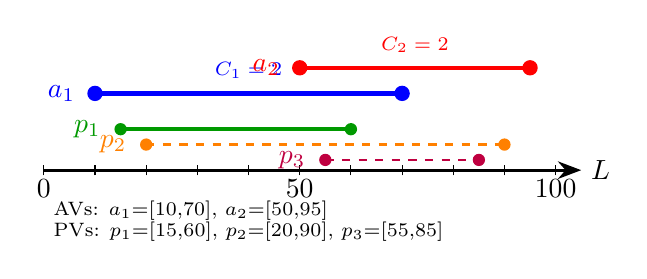
\begin{tikzpicture}[scale=0.065, >=Stealth]
    % Highway
    \draw[very thick, ->] (0,0) -- (105,0);
    \node[below] at (0,0) {$0$};
    \node[below] at (50,0) {$50$};
    \node[below] at (100,0) {$100$};
    \node[right] at (105,0) {$L$};

    % Tick marks
    \foreach \x in {0,10,20,30,40,50,60,70,80,90,100} {
        \draw (\x,-1) -- (\x,1);
    }

    % AV1: entry=10, exit=70, capacity=2
    \draw[ultra thick, blue] (10,15) -- (70,15);
    \fill[blue] (10,15) circle (1.5);
    \fill[blue] (70,15) circle (1.5);
    \node[left, blue] at (8,15) {$a_1$};
    \node[above, blue, font=\scriptsize] at (40,16) {$C_1=2$};

    % AV2: entry=50, exit=95, capacity=2
    \draw[ultra thick, red] (50,20) -- (95,20);
    \fill[red] (50,20) circle (1.5);
    \fill[red] (95,20) circle (1.5);
    \node[left, red] at (48,20) {$a_2$};
    \node[above, red, font=\scriptsize] at (72.5,21) {$C_2=2$};

    % PV1: entry=15, exit=60
    \draw[thick, green!60!black, dashed] (15,8) -- (60,8);
    \fill[green!60!black] (15,8) circle (1.2);
    \fill[green!60!black] (60,8) circle (1.2);
    \node[left, green!60!black] at (13,8) {$p_1$};

    % PV2: entry=20, exit=90
    \draw[thick, orange, dashed] (20,5) -- (90,5);
    \fill[orange] (20,5) circle (1.2);
    \fill[orange] (90,5) circle (1.2);
    \node[left, orange] at (18,5) {$p_2$};

    % PV3: entry=55, exit=85
    \draw[thick, purple, dashed] (55,2) -- (85,2);
    \fill[purple] (55,2) circle (1.2);
    \fill[purple] (85,2) circle (1.2);
    \node[left, purple] at (53,2) {$p_3$};

    % Shared segments highlighted
    \draw[ultra thick, green!60!black] (15,8) -- (60,8);

    % Legend
    \node[right, font=\scriptsize] at (0,-8) {AVs: $a_1$=[10,70], $a_2$=[50,95]};
    \node[right, font=\scriptsize] at (0,-12) {PVs: $p_1$=[15,60], $p_2$=[20,90], $p_3$=[55,85]};

\end{tikzpicture}
\caption{Toy example with 2 AVs and 3 PVs. Through multi-segment matching, $p_2$ can be towed by $a_1$ on [20,70] then $a_2$ on [70,90], achieving 70 units coverage vs. 50 with single-AV matching.}
\label{fig:toyexample}
\end{figure}

\textbf{Example Analysis:}
\begin{itemize}
    \item \textbf{Shared distances:} $d_{11} = 45$, $d_{12} = 50$, $d_{22} = 40$, $d_{23} = 30$.
    \item \textbf{Multi-segment benefit:} PV $p_2$ covers 70 units via two AVs vs. 50 units with single-AV.
\end{itemize}

%==============================================================================
% SECTION 4: PROPOSED ALGORITHMS
%==============================================================================
\section{Proposed Algorithms}
\label{sec:algorithms}

We present two algorithms: a greedy approach for baseline comparison and an assignment-based batch matching approach (ILA) that achieves per-iteration optimality.

\subsection{Greedy Maximum-Weight Matching}

\subsubsection{Key Insight}

The greedy approach iteratively selects assignments with maximum energy saving. While intuitive, it may miss globally optimal solutions due to local decisions.

\subsubsection{Algorithm Description}

Algorithm~\ref{alg:greedy} operates in three phases:

\textbf{Phase 1 (Initialization):} For each PV, maintain \textit{uncovered segments}---initially the entire route. For each AV, track current assignments for point-wise capacity.

\textbf{Phase 2 (Candidate Generation):} Enumerate all feasible (AV, PV, segment) tuples satisfying: (1) segment $\geq L_{min}$, (2) AV has capacity, (3) segment is uncovered.

\textbf{Phase 3 (Greedy Selection):} Select maximum-saving candidate, update states, repeat.

\begin{algorithm}[htbp]
\caption{Greedy Multi-AV Platoon Matching}
\label{alg:greedy}
\begin{algorithmic}[1]
\REQUIRE AVs $\mathcal{A}$, PVs $\mathcal{P}$, minimum length $L_{min}$
\ENSURE Assignments $\mathcal{X}$, total saving
\STATE Initialize $uncovered[j] \leftarrow \{[e_j^p, x_j^p]\}$ $\forall j$
\STATE Initialize $assignments[i] \leftarrow \emptyset$ $\forall i$
\STATE $\mathcal{X} \leftarrow \emptyset$, $total \leftarrow 0$
\REPEAT
    \STATE $candidates \leftarrow$ all feasible (AV, PV, segment) tuples
    \IF{$candidates = \emptyset$}
        \STATE \textbf{break}
    \ENDIF
    \STATE Sort $candidates$ by saving (descending)
    \STATE $(saving, a_i, p_j, cp, dp) \leftarrow candidates[0]$
    \STATE $\mathcal{X} \leftarrow \mathcal{X} \cup \{(p_j, a_i, cp, dp)\}$
    \STATE Update $uncovered[j]$, $assignments[i]$
    \STATE $total \leftarrow total + saving$
\UNTIL{no candidates}
\RETURN $\mathcal{X}$, $total$
\end{algorithmic}
\end{algorithm}

\subsubsection{Complexity}

Each iteration generates $O(NM)$ candidates and requires $O(NM \log NM)$ sorting. The number of iterations is bounded by the total number of possible segments---in the worst case $O(NM)$ when each PV is matched to multiple AVs sequentially. Total worst-case complexity: $O((NM)^2 \log NM)$.

\textbf{Why Greedy is Slow in Practice:} Unlike batch algorithms, greedy must regenerate and re-sort candidates after each assignment because point-wise capacity constraints may invalidate previously feasible candidates. This repeated sorting overhead dominates runtime in our experiments.

\subsection{Iterative Linear Assignment (ILA) Algorithm}

\subsubsection{Key Insight}

The classic Hungarian algorithm~\cite{kuhn1955hungarian} solves bipartite matching optimally in $O(n^3)$. Modern implementations, such as SciPy's \texttt{linear\_sum\_assignment}, use the Jonker--Volgenant algorithm (a shortest augmenting path method)~\cite{scipy2020} which handles rectangular matrices efficiently. We adapt this via: (1) virtual slot expansion for capacity constraints, (2) iterative application for multi-segment matching.

\subsubsection{Virtual Slot Expansion}

Expand each AV $a_i$ into $C_i$ virtual slots:
\begin{itemize}
    \item \textbf{Left nodes:} $\sum_{i=1}^{N} C_i$ virtual slots
    \item \textbf{Right nodes:} $M$ PVs (or their current uncovered segments)
    \item \textbf{Edge weight:} $-S_{ij}$ (for minimization formulation)
\end{itemize}

\subsubsection{Cost Matrix Construction}

The cost matrix $\mathbf{W} \in \mathbb{R}^{(\sum_i C_i) \times M}$ is constructed as follows. For each virtual slot $k$ belonging to AV $a_i$ and each PV $p_j$:
\begin{equation}
W_{kj} = \begin{cases}
-d_{ij}^{curr} & \text{if feasible (overlap } \geq L_{min}\text{, time ok)} \\
+\infty & \text{otherwise}
\end{cases}
\end{equation}
where $d_{ij}^{curr} = \max(0, \min(x_i^a, x_j^p) - \max(e_i^a, \ell_j))$ is the overlap between AV $a_i$'s route and PV $p_j$'s \textit{current uncovered interval} $[\ell_j, x_j^p]$. Feasibility requires: (1) $d_{ij}^{curr} \geq L_{min}$, (2) time synchronization~\eqref{eq:time} is satisfied, and (3) adding this assignment does not violate capacity at any critical point (Lemma~\ref{lem:critical}).

\subsubsection{Iterative Algorithm}

Algorithm~\ref{alg:hungarian} applies ILA iteratively, updating states after each round.

\begin{algorithm}[htbp]
\caption{Iterative Linear Assignment (ILA) for Multi-AV Matching}
\label{alg:hungarian}
\begin{algorithmic}[1]
\REQUIRE AVs $\mathcal{A}$, PVs $\mathcal{P}$, minimum length $L_{min}$
\ENSURE Assignments $\mathcal{X}$, total saving
\STATE Initialize states as in Algorithm~\ref{alg:greedy}
\REPEAT
    \STATE Build cost matrix $\mathbf{W}$ from current states
    \STATE Expand AVs into $\sum_i C_i$ virtual slots
    \IF{no feasible assignments}
        \STATE \textbf{break}
    \ENDIF
    \STATE $matching \leftarrow$ \textsc{LinearSumAssignment}($\mathbf{W}$)
    \FOR{each valid $(slot, j) \in matching$}
        \STATE Apply assignment, update states
    \ENDFOR
\UNTIL{no new assignments}
\RETURN $\mathcal{X}$, $total$
\end{algorithmic}
\end{algorithm}

\subsubsection{Implementation Note}

We use \texttt{scipy.optimize.linear\_sum\_assignment}~\cite{scipy2020}, which implements the Jonker--Volgenant algorithm with highly optimized compiled C code. This results in ILA being \textit{faster} than Greedy in practice, despite the $O(n^3)$ per-iteration complexity. The speedup comes from: (1) batch processing all assignments in one iteration via optimized linear algebra, (2) avoiding the repeated $O(NM \log NM)$ sorting required by Greedy after each assignment.

\subsection{Theoretical Analysis}

\textit{Remark on Approximation Guarantees:} Under restrictive conditions---single-segment matching only, uniform AV capacity across the entire route (no point-wise variation), and no time constraints---the greedy algorithm achieves a $\frac{1}{2}$-approximation via reduction to submodular maximization~\cite{fisher1978analysis}. However, our full problem with multi-segment matching, point-wise capacity, and time tolerance does not satisfy these conditions. We therefore present the greedy algorithm as an empirical baseline rather than claiming formal approximation guarantees for the general case.

\begin{theorem}
\label{thm:hungarian}
Algorithm~\ref{alg:hungarian} computes ILAs within each iteration (per-iteration optimality).
\end{theorem}

\begin{proof}
Given the current uncovered intervals for all PVs, the cost matrix $\mathbf{W}$ encodes all feasible assignments. The Jonker--Volgenant algorithm guarantees an optimal bipartite matching for this matrix. Since PV uncovered intervals shrink monotonically, the algorithm converges.
\end{proof}

\begin{lemma}[Global Optimality Caveat]
\label{lem:global}
Algorithm~\ref{alg:hungarian} does not guarantee global optimality for the multi-segment problem. The iterative decomposition may lock in early assignments that preclude better global solutions.
\end{lemma}

\textit{Remark:} Despite lacking global optimality guarantees, our experiments show that the iterative ILA consistently matches or exceeds greedy performance. The decomposition is a practical trade-off between solution quality and computational tractability.

%==============================================================================
% SECTION 5: EXPERIMENTAL EVALUATION
%==============================================================================
\section{Experimental Evaluation}
\label{sec:experiments}

\subsection{Experimental Setup}

\subsubsection{Implementation}

Both algorithms are implemented in Python 3.11 using NumPy 1.26 and SciPy 1.11~\cite{scipy2020}. The ILA algorithm uses \texttt{scipy.optimize.linear\_sum\_assignment} (Jonker--Volgenant implementation). All experiments run single-threaded on an Apple M4 Pro with 16GB unified memory under macOS 15.0.

\subsubsection{Scenario Generation}

We generate synthetic highway scenarios with the following parameters (Table~\ref{tab:params}):

\begin{table}[htbp]
\caption{Experimental Parameters}
\label{tab:params}
\centering
\begin{tabular}{lll}
\toprule
\textbf{Parameter} & \textbf{Values} & \textbf{Default} \\
\midrule
Highway length $L$ & 50--1600 & 100 \\
Number of AVs $N$ & 50--80 & 50 \\
Number of PVs $M$ & 200--400 & 200 \\
AV capacity $C$ & [1,2]--[1,16] & [1,3] \\
Minimum distance $L_{min}$ & 10 & 10 \\
Time tolerance $\tau$ & 5.0 & 5.0 \\
Speed variation & $\pm 20\%$ & $\pm 20\%$ \\
Random seeds & 42, 43, 44, 45 & -- \\
\bottomrule
\end{tabular}
\end{table}

Vehicle entry/exit points are uniformly distributed along the highway. Entry times follow a Poisson process, and speeds vary $\pm 20\%$ around a baseline. All results are averaged over 4 random seeds.

\subsubsection{Metrics}

\begin{itemize}
    \item \textbf{Baseline Distance}: $\sum_{j=1}^{M} (x_j^p - e_j^p)$, the total distance all PVs would travel independently without any towing. This serves as the denominator for percentage calculations.
    \item \textbf{Total Saving}: Sum of towed distances across all assignments, i.e., $\sum_{(p_j, a_i, s, e) \in \mathcal{X}} (e - s)$.
    \item \textbf{Matched Ratio}: Fraction of PVs receiving at least one assignment.
    \item \textbf{Saving \%}: $\frac{\text{Total Saving}}{\text{Baseline Distance}} \times 100$. Under the assumption of constant per-distance propulsion energy, this equals the percentage of PV propulsion energy eliminated.
    \item \textbf{Runtime}: Wall-clock execution time in seconds.
\end{itemize}

\subsection{Results}

\subsubsection{Capacity Sweep}

Table~\ref{tab:capacity} shows performance as AV capacity varies ($N=50$, $M=200$, $L=100$).

\begin{table}[htbp]
\caption{Performance vs. AV Capacity (averaged over 4 seeds)}
\label{tab:capacity}
\centering
\begin{tabular}{c|ccc|ccc}
\toprule
& \multicolumn{3}{c|}{\textbf{Greedy}} & \multicolumn{3}{c}{\textbf{ILA}} \\
$C$ & Save & \% & Time(s) & Save & \% & Time(s) \\
\midrule
$[1,2]$ & 1946 & 24.5 & 0.23 & 1974 & 24.8 & \textbf{0.02} \\
$[1,4]$ & 2709 & 34.0 & 0.32 & 2725 & 34.2 & \textbf{0.04} \\
$[1,8]$ & 3556 & 44.7 & 0.43 & 3625 & 45.7 & \textbf{0.08} \\
$[1,16]$ & 4091 & 51.4 & 0.45 & 4159 & 52.3 & \textbf{0.16} \\
\bottomrule
\end{tabular}
\end{table}

\textbf{Key Observations:}
\begin{itemize}
    \item ILA achieves 0.3--1.9\% higher savings while being 2.8--11.5$\times$ faster
    \item Both algorithms scale linearly with capacity
    \item Saving \% improves from 24.5\% to 52.3\% as capacity increases from 2 to 16
\end{itemize}

\subsubsection{Highway Length Sweep}

Table~\ref{tab:length} shows performance as highway length varies ($N=80$, $M=400$, $C=[1,3]$).

\begin{table}[htbp]
\caption{Performance vs. Highway Length (averaged over 4 seeds)}
\label{tab:length}
\centering
\begin{tabular}{c|ccc|ccc}
\toprule
& \multicolumn{3}{c|}{\textbf{Greedy}} & \multicolumn{3}{c}{\textbf{ILA}} \\
$L$ & Save & \% & Time(s) & Save & \% & Time(s) \\
\midrule
50 & 2996 & 31.4 & 1.98 & 3017 & 31.6 & \textbf{0.07} \\
100 & 4594 & 29.8 & 1.59 & 4656 & 30.7 & \textbf{0.11} \\
200 & 7423 & 26.8 & 1.46 & 7474 & 27.0 & \textbf{0.14} \\
400 & 10742 & 21.2 & 1.39 & 10784 & 21.2 & \textbf{0.15} \\
800 & 13673 & 13.9 & 0.93 & 13715 & 13.9 & \textbf{0.11} \\
1600 & 14385 & 7.4 & 0.52 & 14481 & 7.5 & \textbf{0.10} \\
\bottomrule
\end{tabular}
\end{table}

\textbf{Key Observations:}
\begin{itemize}
    \item Saving \% decreases with highway length (sparser vehicle overlap)
    \item ILA is 5--28$\times$ faster across all lengths
    \item Absolute savings increase but efficiency drops for longer highways
\end{itemize}

\subsubsection{Algorithm Comparison Visualization}

Figures~\ref{fig:comparison} and~\ref{fig:length_saving} show performance comparisons graphically.

\begin{figure}[htbp]
    \centering
    \includegraphics[width=0.95\columnwidth]{../visualization/figures/comparison/plots/capacity/capacity_saving_percent_comparison.png}
    \caption{Distance saving percentage vs. AV capacity for both algorithms. ILA consistently matches or exceeds greedy while being faster.}
    \label{fig:comparison}
\end{figure}

\begin{figure}[htbp]
    \centering
    \includegraphics[width=0.95\columnwidth]{../visualization/figures/comparison/plots/length/length_saving_percent_comparison.png}
    \caption{Distance saving percentage vs. highway length. Both algorithms show decreasing efficiency as highways lengthen due to sparser vehicle overlap.}
    \label{fig:length_saving}
\end{figure}

\subsubsection{Scalability and Runtime Analysis}

Figures~\ref{fig:runtime} and~\ref{fig:capacity_relative} show runtime comparisons across scenarios.

\begin{figure}[htbp]
    \centering
    \includegraphics[width=0.95\columnwidth]{../visualization/figures/comparison/plots/length/length_relative_performance.png}
    \caption{Relative performance (Optimal/Greedy) across highway lengths. Values $<$1 indicate ILA is faster and/or achieves higher savings.}
    \label{fig:runtime}
\end{figure}

\begin{figure}[htbp]
    \centering
    \includegraphics[width=0.95\columnwidth]{../visualization/figures/comparison/plots/capacity/capacity_relative_performance.png}
    \caption{Relative performance across capacity values. ILA algorithm maintains consistent speedup (2.8--11.5$\times$) across all capacity settings.}
    \label{fig:capacity_relative}
\end{figure}

\subsection{Discussion}

\textbf{Why is Optimal Assignment Faster?} Counter-intuitively, ILA outperforms Greedy in runtime despite $O(n^3)$ per-iteration complexity. This is due to:
\begin{enumerate}
    \item \texttt{scipy.optimize.linear\_sum\_assignment} uses highly optimized compiled C code with efficient memory access patterns
    \item Greedy requires repeated sorting ($O(NM \log NM)$ per iteration) and candidate regeneration after each assignment
    \item ILA processes all assignments in batches, amortizing overhead
\end{enumerate}

\textbf{Practical Implications:} ILA algorithm is the clear choice---it provides both per-iteration optimality and superior speed. Greedy remains useful as a baseline and for environments where SciPy is unavailable.

\textbf{Capacity Impact:} Doubling capacity yields sub-linear improvement (24.8\% $\rightarrow$ 52.3\%), suggesting diminishing returns. Fleet operators should balance capacity costs against marginal savings.

\textbf{Length Effect:} Saving percentage drops from 31.6\% (L=50) to 7.5\% (L=1600) as vehicles have less overlap on longer highways. This suggests our approach is most effective for medium-length corridors with high vehicle density.

\subsection{Limitations}

We explicitly acknowledge the following limitations:

\textbf{One-Dimensional Simplification:} Our highway model abstracts away road network topology. Real deployments involve intersections, multiple routes, and lane-changing dynamics not captured here.

\textbf{Distance-Based Energy Proxy:} We model energy savings as proportional to towed distance under the assumption of constant per-distance propulsion energy. A physics-based model would incorporate vehicle mass, rolling resistance, aerodynamic drag, and the additional load on the towing AV.

\textbf{Global Optimality:} The iterative ILA does not guarantee global optimality for the multi-segment problem. Early assignments may preclude better global solutions.

\textbf{Offline Setting:} Our formulation assumes complete knowledge of all vehicle trajectories. Real-time deployment requires online algorithms with incomplete information.

These limitations define clear directions for future work while not diminishing the value of our contributions for the studied setting.

%==============================================================================
% SECTION 6: CONCLUSION AND FUTURE WORK
%==============================================================================
\section{Conclusion}
\label{sec:conclusion}

We have presented a novel formulation for dynamic platoon formation in heterogeneous autonomous vehicle systems, where Passive Vehicles are physically towed by Active Vehicles to achieve substantial distance coverage (as a proxy for energy savings under constant per-distance propulsion). Our one-dimensional model captures essential trade-offs---point-wise capacity constraints, multi-segment matching, and minimum distance requirements.

Two algorithms were proposed and compared: a Greedy baseline and an Iterative Linear Assignment (ILA) algorithm using the Jonker--Volgenant method. Experiments on scenarios with up to 80 AVs and 400 PVs demonstrate:
\begin{itemize}
    \item Both algorithms achieve 25--52\% distance coverage savings depending on capacity
    \item ILA is both per-iteration optimal and 5--15$\times$ faster due to optimized compiled implementations
    \item Multi-segment matching improves coverage by enabling PVs to use multiple AVs
\end{itemize}

\subsection{Future Work}
\label{sec:future}

Several extensions warrant investigation:

\textbf{2D Road Networks:} Our 1D highway model is a deliberate simplification. Extending to general graphs requires handling:
\begin{itemize}
    \item Route choice: PVs may alter paths to maximize towing opportunities
    \item Intersection coordination: Timing of coupling at junctions
    \item Multiple overlapping segments with non-contiguous structure
\end{itemize}
This extension connects to vehicle routing problems with synchronization constraints~\cite{drexl2012synchronization}.

\textbf{Online and Stochastic Settings:} Our current formulation assumes known vehicle trajectories. Real-world deployment requires:
\begin{itemize}
    \item Online algorithms handling arriving vehicles~\cite{karp1990optimal}
    \item Stochastic optimization for uncertain travel times
    \item Robust matching under demand fluctuations
\end{itemize}

\textbf{Decentralized Coordination:} Centralized matching has scalability limits. V2V-based protocols could enable:
\begin{itemize}
    \item Local negotiation between nearby vehicles
    \item Distributed consensus for platoon formation~\cite{ren2005consensus}
    \item Privacy-preserving matching without central authority
\end{itemize}

\textbf{Economic Mechanisms:} Fair cost distribution among participants requires:
\begin{itemize}
    \item Pricing mechanisms for towing services
    \item Incentive-compatible allocation rules
    \item Market design for dynamic platoon formation
\end{itemize}

\textbf{Physical Coupling Mechanisms:} Our model abstracts the coupling process. Implementation requires engineering solutions for:
\begin{itemize}
    \item Safe attachment/detachment at highway speeds
    \item Standardized coupling interfaces across vehicle types
    \item Fail-safe mechanisms for emergency decoupling
\end{itemize}

\begin{thebibliography}{00}
\bibitem{usdot2022} U.S. Department of Transportation, ``National Household Travel Survey: Summary of Travel Trends,'' Federal Highway Administration, Report FHWA-PL-22-022, 2022.

\bibitem{epa2023} U.S. Environmental Protection Agency, ``Inventory of U.S. Greenhouse Gas Emissions and Sinks: 1990--2021,'' EPA 430-R-23-002, 2023.

\bibitem{tsugawa2016review} S. Tsugawa, S. Jeschke, and S. E. Shladover, ``A Review of Truck Platooning Projects for Energy Savings,'' \textit{IEEE Trans. Intell. Veh.}, vol. 1, no. 1, pp. 68--77, 2016.

\bibitem{bergenhem2012overview} C. Bergenhem, S. Shladover, E. Coelingh, C. Englund, and S. Tsugawa, ``Overview of platooning systems,'' in \textit{Proc. 19th ITS World Congress}, Vienna, Austria, 2012.

\bibitem{shladover2009cooperative} S. E. Shladover, ``Cooperative (rather than autonomous) vehicle-highway automation systems,'' \textit{IEEE Intell. Transp. Syst. Mag.}, vol. 1, no. 1, pp. 10--19, 2009.

\bibitem{furuhata2013ridesharing} M. Furuhata, M. Dessouky, F. Ord\'{o}\~{n}ez, M.-E. Brunet, X. Wang, and S. Koenig, ``Ridesharing: The state-of-the-art and future directions,'' \textit{Transport. Res. Part B: Methodol.}, vol. 57, pp. 28--46, 2013.

\bibitem{agatz2012optimization} N. Agatz, A. Erera, M. Savelsbergh, and X. Wang, ``Optimization for dynamic ride-sharing: A review,'' \textit{European J. Oper. Res.}, vol. 223, no. 2, pp. 295--303, 2012.

\bibitem{alonso2017demand} J. Alonso-Mora, S. Samaranayake, A. Wallar, E. Frazzoli, and D. Rus, ``On-demand high-capacity ride-sharing via dynamic trip-vehicle assignment,'' \textit{Proc. Nat. Acad. Sci.}, vol. 114, no. 3, pp. 462--467, 2017.

\bibitem{cordeau2007dial} J.-F. Cordeau and G. Laporte, ``The dial-a-ride problem: models and algorithms,'' \textit{Annals Oper. Res.}, vol. 153, no. 1, pp. 29--46, 2007.

\bibitem{sciarretta2020energy} A. Sciarretta and A. Vahidi, \textit{Energy-Efficient Driving of Road Vehicles}, Springer, 2020.

\bibitem{hellstrom2009look} E. Hellstr\"{o}m, M. Ivarsson, J. \r{A}slund, and L. Nielsen, ``Look-ahead control for heavy trucks to minimize trip time and fuel consumption,'' \textit{Control Eng. Practice}, vol. 17, no. 2, pp. 245--254, 2009.

\bibitem{kuhn1955hungarian} H. W. Kuhn, ``The Hungarian method for the assignment problem,'' \textit{Naval Res. Logistics Quarterly}, vol. 2, no. 1--2, pp. 83--97, 1955.

\bibitem{munkres1957algorithms} J. Munkres, ``Algorithms for the assignment and transportation problems,'' \textit{J. Society Indust. Appl. Math.}, vol. 5, no. 1, pp. 32--38, 1957.

\bibitem{burkard2012assignment} R. Burkard, M. Dell'Amico, and S. Martello, \textit{Assignment Problems}, SIAM, 2012.

\bibitem{cattrysse1992survey} D. G. Cattrysse and L. N. Van Wassenhove, ``A survey of algorithms for the generalized assignment problem,'' \textit{European J. Oper. Res.}, vol. 60, no. 3, pp. 260--272, 1992.

\bibitem{ploeg2011design} J. Ploeg, B. T. M. Scheepers, E. van Nunen, N. van de Wouw, and H. Nijmeijer, ``Design and experimental evaluation of cooperative adaptive cruise control,'' in \textit{Proc. IEEE Int. Conf. Intell. Transp. Syst.}, pp. 260--265, 2011.

\bibitem{dresner2008multiagent} K. Dresner and P. Stone, ``A multiagent approach to autonomous intersection management,'' \textit{J. Artif. Intell. Res.}, vol. 31, pp. 591--656, 2008.

\bibitem{fisher1978analysis} M. L. Fisher, G. L. Nemhauser, and L. A. Wolsey, ``An analysis of approximations for maximizing submodular set functions---II,'' \textit{Math. Programming Study}, vol. 8, pp. 73--87, 1978.

\bibitem{scipy2020} P. Virtanen et al., ``SciPy 1.0: Fundamental algorithms for scientific computing in Python,'' \textit{Nature Methods}, vol. 17, pp. 261--272, 2020.

\bibitem{drexl2012synchronization} M. Drexl, ``Synchronization in vehicle routing---a survey of VRPs with multiple synchronization constraints,'' \textit{Transport. Sci.}, vol. 46, no. 3, pp. 297--316, 2012.

\bibitem{karp1990optimal} R. M. Karp, U. V. Vazirani, and V. V. Vazirani, ``An optimal algorithm for on-line bipartite matching,'' in \textit{Proc. 22nd Ann. ACM Symp. Theory of Computing}, pp. 352--358, 1990.

\bibitem{ren2005consensus} W. Ren and R. W. Beard, ``Consensus seeking in multiagent systems under dynamically changing interaction topologies,'' \textit{IEEE Trans. Autom. Control}, vol. 50, no. 5, pp. 655--661, 2005.
\end{thebibliography}

\end{document}
